\begin{figure}
\centering
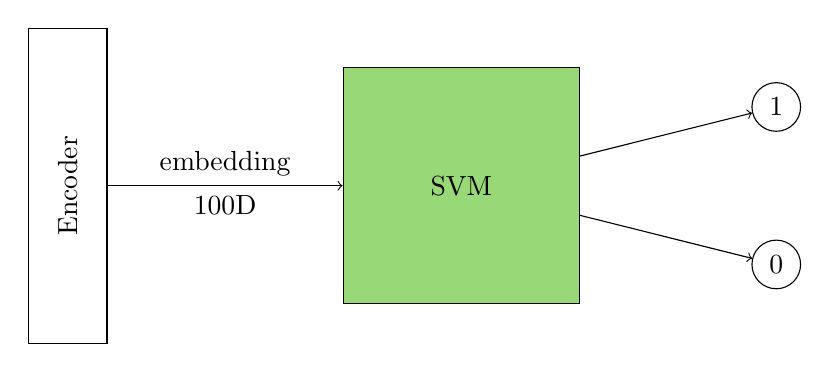
\begin{tikzpicture}

\node (ed) [draw, rectangle, minimum width=1cm, minimum height=4cm, text centered] {\rotatebox{90}{Encoder}};

\node (svm) [draw, rectangle, text centered, right of=ed, node distance=5cm, minimum height=3cm, minimum width=3cm, fill=yellow!60!cyan] {SVM};


\node (class1) [draw, circle,right of=svm, node distance=4cm, text centered, yshift=-1cm ] {0};
\node (class2) [draw, circle,right of=svm, node distance=4cm, text centered, yshift=1cm] {1};

\draw[->] (ed) -- (svm) node[midway, above] {embedding} node[midway, below] {100D};
\draw[->] (svm) -- (class1);
\draw[->] (svm) -- (class2);


\end{tikzpicture}
\end{figure}
